\documentclass[manuscript,review]{acmart}
%%
%% \BibTeX command to typeset BibTeX logo in the docs
\AtBeginDocument{%
  \providecommand\BibTeX{{%
    Bib\TeX}}}
\setcopyright{none}
\settopmatter{printacmref=false, printfolios=true}
\begin{document}

%% The "title" command has an optional parameter,
%% allowing the author to define a "short title" to be used in page headers.
\title{Local-First: Human-Centered  Routing Between Local and Frontier Language Models}

%% The "author" command and its associated commands are used to define
%% the authors and their affiliations.
%% Of note is the shared affiliation of the first two authors, and the
%% "authornote" and "authornotemark" commands
%% used to denote shared contribution to the research.
\author{Kaleb Flowers}
\email{KalebFlowers@colostate.edu}
\affiliation{%
  \institution{Colorado State University}
  \city{Fort Collins}
  \state{Colorado}
  \country{USA}
}

%%
%% By default, the full list of authors will be used in the page
%% headers. Often, this list is too long, and will overlap
%% other information printed in the page headers. This command allows
%% the author to define a more concise list
%% of authors' names for this purpose.
\renewcommand{\shortauthors}{Flowers}

%%
%% The abstract is a short summary of the work to be presented in the
%% article.
\begin{abstract}
As language models become increasingly available through both local inference and cloud-based services, understanding how users perceive and evaluate their outputs becomes important to the development of human-centered AI systems. This study investigates whether model-source attribution influences human evaluation of AI-generated Python code. A within-subjects experiment was conducted with 12 participants, each evaluating four programming solutions presented under Local and Frontier model-source labels. Evaluation accuracy, confidence, and subjective workload were examined using Bayesian statistical models. Participants demonstrated higher evaluation accuracy under the Local condition (83.33\%) than under the Frontier condition (70.83\%), while differences in confidence and subjective workload were comparatively small. An exploratory analysis also indicated that participants were more likely to classify Local-labeled solutions as correct, regardless of actual solution correctness. However, all 95\% credible intervals included their respective null values, indicating substantial uncertainty in the estimated effects. These findings provide preliminary evidence that model-source attribution may influence how users evaluate AI-generated code and highlight the importance of considering human perceptions when developing systems that incorporate local language models.
\end{abstract}

%%
%% The code below is generated by the tool at http://dl.acm.org/ccs.cfm.
%% Please copy and paste the code instead of the example below.
%%
\begin{CCSXML}

\end{CCSXML}


%%
%% Keywords. The author(s) should pick words that accurately describe
%% the work being presented. Separate the keywords with commas.
\keywords{human-centered AI; human-AI interaction; trust in AI; source attribution bias; code correctness evaluation; local language models; frontier language models; cognitive workload}
%% A "teaser" image appears between the author and affiliation
%% information and the body of the document, and typically spans the
%% page.

%%
%% This command processes the author and affiliation and title
%% information and builds the first part of the formatted document.
\maketitle


\section{Introduction}

Large language models are increasingly available through both powerful cloud services and smaller models that can run directly on consumer hardware. Frontier models provide strong performance across a wide range of tasks, but relying on them comes with costs in energy consumption, privacy, network dependence, and monetary expense. Smaller language models require fewer computational resources and can operate locally, potentially reducing some of these costs. However, the usefulness of local models depends not only on their technical capabilities but also on how users perceive and evaluate the results they produce. Users may perceive frontier models as more capable or reliable simply because of their source, even when a smaller model can produce a satisfactory result.

This raises an important question about how users evaluate AI-generated content. When reviewing code, users must determine whether a solution correctly satisfies the requirements of a programming problem. Their judgments may be influenced by expectations about the model that produced the code rather than the code itself. This study investigates whether labeling AI-generated Python code as originating from a Local or Frontier model influences evaluation accuracy, confidence, and subjective workload. A within-subjects experiment was conducted in which participants evaluated programming solutions under both model-source labels and reported their confidence and perceived workload following each evaluation. The study also examines whether model-source labels influence participants' tendency to classify programming solutions as correct, regardless of their actual correctness. By examining the relationship between model-source attribution and human evaluation, this research aims to better understand the role of perceived model capability in human-AI interaction and inform the development of systems that incorporate local language models.



% --------------------------------------------------
\section{Related Work}
\noindent\textbf{Local and Cloud Inference}\par
\noindent Research on smaller language models has demonstrated that useful capabilities are not limited to the largest cloud-based systems. MobileLLM demonstrates that sub-billion-parameter language models can be optimized for on-device applications while maintaining competitive performance on selected tasks~\cite{liu2024mobilellm}. Jeanquartier et al. examine the resource and environmental effects of language-model deployment and identify potential sustainability benefits of smaller models, although efficiency depends on the model, hardware, and workload~\cite{jeanquartier2026carbon}. These studies establish the practical motivation for local inference, but they primarily examine model performance and resource requirements rather than how users perceive locally generated outputs.

\noindent\textbf{Adaptive LLM Routing}\par
\noindent Previous research has investigated how to select between language models with different capabilities and computational costs. FrugalGPT uses a cascading approach where models are called sequentially and responses are evaluated before deciding whether a more expensive model is needed~\cite{chen2024frugalgpt}. Hybrid LLM instead makes the routing decision before inference by predicting whether a smaller model can provide sufficient response quality~\cite{ding2024hybridllm}. RouteLLM trains routing models using human preference data to select between weaker and stronger models~\cite{ong2025routellm}. BEST-Route extends this approach by considering both model selection and the amount of test-time computation allocated to a request~\cite{ding2025bestroute}. Pozi and Sato apply routing specifically to program generation, using a lightweight classifier to select between edge and cloud models~\cite{pozi2025routing}. Together, these approaches demonstrate methods for reducing reliance on larger models while maintaining response quality. However, their primary focus is on automated model selection rather than how users evaluate outputs attributed to different models.

\noindent\textbf{Model Source Labels and Human Evaluation}\par
\noindent Information about the source of AI-generated content may influence how users evaluate its reliability. Sun et al. investigate the effects of source labels on trust assessments made by humans and LLM-based evaluators. Their study compares evaluations of identical content presented under different source labels, demonstrating that source attribution can influence trust judgments even when the underlying content remains unchanged~\cite{sun-etal-2026-label}. This suggests that users may rely on expectations about the source of information when evaluating AI-generated outputs rather than relying exclusively on the content itself.

While Sun et al. examine Human and AI source labels, the present study investigates differences within AI-generated content by comparing Local and Frontier model labels. Rather than assessing the general trustworthiness of information, participants evaluate whether Python solutions correctly satisfy programming requirements. The experiment measures correctness judgment accuracy, confidence, and subjective workload while varying the perceived model source. This extends the investigation of source-label effects into programming tasks, where participants must evaluate the functional correctness of generated code rather than simply assess the credibility of a response.
% --------------------------------------------------


% --------------------------------------------------
\section{System}

The experimental system was implemented using Qualtrics, a web-based survey platform that supports randomized experimental conditions and structured response collection. The survey was organized into three main components: a background questionnaire, programming evaluation tasks, and a final questionnaire. Eight Python programming problems were incorporated into the survey, each containing a problem description, a proposed solution, and a model-source label. The interface was designed for remote participation and required no additional software installation. A remote, self-administered format was selected to reduce barriers to participation and eliminate the need to schedule individual sessions or travel to a designated location.

Qualtrics' randomization features were used to select four of the eight programming problems for each participant, including two from each difficulty category. Programming evaluations were organized into two blocks containing two problems each. One block was assigned the Local model-source label and the other was assigned the Frontier label, with the presentation order randomized across participants. Each programming problem was presented using a consistent layout, with the model-source label visually emphasized to ensure that participants could identify the attributed source. The problem description and Python solution were displayed separately to make the requirements and accompanying code easier to distinguish.

Participant responses were collected directly through Qualtrics following each programming problem. Each evaluation recorded a correctness judgment, a five-point confidence rating, and responses to the six NASA-TLX workload dimensions. The survey also collected participant background information and a final response regarding the use of external assistance. Qualtrics associated responses with unique response identifiers and recorded the randomized problem selections and model-source assignments. The collected data were exported as CSV files for subsequent statistical analysis using Python.

% --------------------------------------------------

% --------------------------------------------------
\section{Method}
\subsection{Study Design}
A controlled, within-subjects experiment was conducted to investigate how perceived model origin influenced participants' evaluations of AI-generated programming solutions. The independent variable was the model-source label, with two experimental conditions: Local and Frontier. The study examined whether these labels influenced participants' ability to identify correct and incorrect programming solutions, their confidence in those judgments, and their perceived workload. The within-subjects design allowed comparisons within individual participants while reducing the influence of differences in programming experience. Participants evaluated existing solutions rather than writing or modifying code, allowing the experiment to focus on correctness judgments rather than programming task completion.

Eight Python programming problems were developed, and each participant evaluated four: two easy-to-moderate problems and two moderately difficult problems. The problem pool contained four correct and four incorrect solutions. Problems were selected through Qualtrics randomization, and evaluations were organized into two blocks containing two programming problems each. Model-source labels were assigned at the block level, with one block labeled Local and the other labeled Frontier. The presentation order of the two conditions was randomized across participants. Labels were assigned independently of the actual model used to generate the code, allowing the same programming solution to be evaluated under different labels across participants. Following each programming problem, participants provided a correctness judgment and a five-point confidence rating and were presented with the Raw NASA Task Load Index (NASA-TLX) questionnaire.

\subsection{Participants and Ethics}

A total of 12 participants completed the experiment, meeting the minimum recruitment target established for the study. This included one participant who completed an earlier pilot version of the experiment. All 12 participants were retained for the analysis of evaluation accuracy and confidence, while 11 participants were included in the subjective workload analysis due to missing NASA-TLX assessments in the pilot response. A sensitivity analysis was conducted to assess the influence of including the pilot participant. Participants were recruited through convenience sampling, primarily from the Colorado State University computer science community. Participation was entirely voluntary, and eligibility required sufficient programming knowledge to independently read and evaluate code involving fundamental programming concepts, control structures, and basic data structures. Programming ability was self-reported, and no additional competency assessment was required.

Before beginning the programming evaluations, participants completed a background questionnaire documenting their academic or professional standing, years of programming experience, familiarity with Python, overall programming proficiency, and frequency of AI coding assistant use. These measures were collected to characterize the participant population and provide context for interpreting evaluation performance and subjective workload. Participants completed the experiment remotely and independently through a single Qualtrics survey link.

\subsubsection{Ethics and Informed Consent}
Participants were provided with information explaining the general purpose of the study, its procedures, estimated completion time of approximately 20 minutes, and the intended use of collected data. Participation was voluntary, and participants could discontinue the experiment without penalty. All 12 participants provided informed consent before beginning the programming evaluations. Responses were associated with unique Qualtrics response identifiers rather than names or other direct personal identifiers. Because model-source labels were experimentally assigned rather than representing the actual source of the solutions, participants received a debriefing explaining the labeling manipulation after completing their evaluations.

\subsection{Materials and Tasks}

The experiment used eight Python programming problems divided into two difficulty categories: four easy-to-moderate and four moderately difficult problems. The problems covered common programming concepts, including lists, strings, loops, conditionals, dictionaries, and basic algorithms. Python was selected for its readability and widespread use in introductory computer science education. Each problem included a brief description of the expected behavior and an AI-generated solution. The programs were kept relatively short, used conventional formatting and clear variable names, and avoided unnecessarily complex logic. Difficulty was determined by the reasoning required to evaluate the code rather than program length or familiarity with specialized algorithms.

All eight solutions were generated using a single AI model to maintain consistency across the experimental materials. Each solution was verified against its problem specification using predefined test cases. Following verification, four solutions were deliberately modified to introduce logical errors while preserving valid Python syntax. The modified solutions were tested again to confirm that the errors affected their correctness. This produced four correct and four incorrect solutions distributed across both difficulty categories. Participants were not informed of the distribution of correct and incorrect solutions.

Each participant evaluated four solutions selected through Qualtrics randomization, with two problems from each difficulty category. The evaluations were organized into two blocks containing two problems each, with one block assigned the Local label and the other assigned the Frontier label. The finalized programming solutions remained identical across presentations regardless of their assigned model-source label. The problems were designed to require logical inspection without relying on obscure errors, misleading formatting, or specialized programming knowledge. All experimental materials were presented through Qualtrics using a standardized format and were designed to support an estimated completion time of approximately 20 minutes.


\subsection{Experimental Procedure}

The experiment was conducted remotely through Qualtrics. Participants accessed the study through a single survey link, reviewed the study information, provided informed consent, and completed the background questionnaire. Qualtrics randomly selected four programming problems from the eight-problem pool, with two problems from each difficulty category. The evaluations were organized into two blocks, each containing two programming problems under the same model-source label. The presentation order of the Local and Frontier conditions was randomized across participants. Participants were provided with brief, neutral descriptions of Local and Frontier language models to establish a common understanding of the terminology. Local models were described as models operating on a user's device, while frontier models were described as representing leading AI capabilities and typically being accessed through cloud-based services. No specific model names were provided, and neither category was presented as inherently more reliable.

Participants were instructed to evaluate each solution independently using their own programming knowledge, without executing the code or consulting AI assistants, search engines, or other external resources. Scratch paper was permitted for manually tracing program execution. For each programming problem, participants were presented with the model-source label, a description of the expected behavior, and the accompanying Python solution. Participants classified the solution as either Correct or Incorrect, rated their confidence using a five-point scale, and completed the Raw NASA-TLX questionnaire to assess their perceived workload. This procedure was repeated across all four programming problems without feedback regarding solution correctness. Participants were informed that the experiment would take approximately 20 minutes, but no time limit was imposed.

At the end of the experiment, participants reported whether they had used external assistance and received a debriefing explaining the experimental labeling manipulation. The use of prohibited external resources was established as an exclusion criterion, although no participants reported using such resources.


\subsection{Measures}

The study used three primary dependent measures to examine how perceived model origin influenced participants' evaluations: evaluation accuracy, evaluation confidence, and subjective workload. Evaluation accuracy served as the primary dependent variable, while confidence and workload captured subjective aspects of the evaluation experience. These measures were collected following each programming problem, allowing responses to be compared between the Local and Frontier conditions. An additional exploratory measure, perceived correctness, was derived from participants' correctness judgments.

\subsubsection{Evaluation Accuracy}

Evaluation accuracy was measured by asking participants to classify each programming solution as either correct or incorrect. Responses were compared against a verified answer key established during the development of the programming problems. Each classification was recorded as accurate or inaccurate based on whether the participant's judgment matched the verified solution status. Accuracy was calculated as the proportion of accurately classified solutions within each model-source condition. Because each participant evaluated two solutions under each label, individual condition-level accuracy scores ranged from 0\% to 100\% in increments of 50 percentage points. Individual classification responses were retained for statistical analysis rather than relying exclusively on aggregated accuracy scores.

\subsubsection{Evaluation Confidence}

Evaluation confidence was measured using a five-point rating scale administered immediately after each correctness judgment. Participants indicated how confident they were in their assessment, ranging from 1 (not confident) to 5 (very confident). Confidence ratings were recorded for each programming solution and averaged separately for the Local and Frontier conditions for descriptive analysis. Individual ratings were retained as ordinal observations for statistical modeling. This measure allowed the study to examine whether model-source labels influenced participants' confidence in their evaluations independently of whether their correctness judgments were accurate.

\subsubsection{Subjective Workload --- NASA-TLX}

Subjective workload was measured using the Raw NASA Task Load Index (NASA-TLX), a standardized questionnaire designed to assess perceived workload during task performance. The instrument evaluated six dimensions: mental demand, physical demand, temporal demand, perceived performance, effort, and frustration. Raw NASA-TLX was selected because it provided an overall workload measure without requiring the additional pairwise comparisons used in the original weighted version. The questionnaire was administered through Qualtrics following each programming problem, using six rating scales ranging from 0 to 100 in increments of five.

An overall subjective workload score was calculated for each completed assessment by taking the arithmetic mean of the six ratings, with higher scores indicating greater perceived workload. Problem-level scores were averaged separately for the Local and Frontier conditions. Although all six dimensions were recorded, the workload analysis focused on the overall score rather than individual dimensions. Only participants with complete workload assessments under both conditions were included in the paired statistical analysis.

\subsubsection{Perceived Correctness}

Perceived correctness was examined as an exploratory measure representing participants' tendency to classify programming solutions as correct regardless of their actual correctness. Unlike evaluation accuracy, this measure did not assess whether the participant's judgment matched the verified solution status. Perceived correctness was calculated as the proportion of solutions classified as correct within each model-source condition. This distinction allowed the analysis to explore whether model-source labels influenced participants' willingness to accept a programming solution as correct rather than solely their ability to evaluate its functional correctness.


\subsection{Data Analysis}
Experimental data were collected through Qualtrics and exported as CSV files for analysis using Python. The analysis used pandas for data preparation, PyMC for Bayesian statistical modeling, ArviZ for model diagnostics, and Matplotlib for visualization. Each response was associated with a unique participant identifier, allowing evaluations from the Local and Frontier conditions to be compared within participants. The dataset was organized with one observation per programming evaluation, producing 48 observations across 12 participants. Each observation contained the programming problem identifier, assigned model-source label, presentation block, verified solution correctness, participant correctness judgment, confidence rating, and NASA-TLX responses.

Before analysis, responses were reviewed for completeness, duplicate response identifiers, participant eligibility, and compliance with the experimental procedure. Experimental assignments were checked to verify that each participant received four programming problems, with two under each model-source label. Correctness judgments were compared against the verified answer key and coded as accurate or inaccurate, while confidence ratings were retained on their original five-point scale. Overall NASA-TLX scores were calculated for each problem by averaging the six workload dimensions. One participant who completed an earlier pilot version of the experiment was retained for the analysis of comparable measurements. This participant was excluded from the paired workload analysis because two NASA-TLX assessments were missing.

The primary statistical analysis used a Bayesian framework to estimate the influence of model-source labels on evaluation accuracy, confidence, and subjective workload. Bayesian methods were selected to estimate the magnitude and uncertainty of potential labeling effects rather than relying exclusively on traditional significance testing. Evaluation accuracy, the primary dependent variable, was analyzed using Bayesian hierarchical logistic regression to estimate the relationship between model-source labels and the probability of correctly classifying a programming solution. Participant-level and problem-level random intercepts accounted for repeated observations and differences between individual programming problems. Actual solution correctness and presentation block were included as additional predictors.

Evaluation confidence was analyzed using Bayesian hierarchical ordinal logistic regression to account for the ordered five-point response scale. The model included the same predictors and random effects as the evaluation accuracy model. Subjective workload was analyzed using a Bayesian paired-difference model comparing each participant's average NASA-TLX scores under the Local and Frontier conditions. The workload analysis included the 11 participants with complete measurements under both conditions. An additional exploratory Bayesian hierarchical logistic regression examined perceived correctness, defined as the probability of classifying a solution as correct regardless of whether that classification was accurate.

Weakly informative normal priors with a mean of zero and a standard deviation of 1.5 were specified for the regression coefficients. Half-normal priors with a scale of 1 were specified for the participant-level and problem-level random-effect standard deviations. The ordinal regression used four ordered thresholds with normal priors centered at zero and a standard deviation of 2.5. For the paired workload model, a normal prior centered at zero with a standard deviation of 20 was specified for the mean difference, and a half-normal prior with a scale of 20 was specified for the residual standard deviation.

Posterior distributions were estimated using the No-U-Turn Sampler (NUTS) implemented in PyMC. Each model was fitted using four independent sampling chains with 4,000 retained posterior draws per chain, producing 16,000 posterior samples per model. Between 2,000 and 3,000 tuning iterations were used per chain, with target acceptance probabilities ranging from 0.95 to 0.99. Model convergence was assessed using rank-normalized $\hat{R}$ statistics, bulk and tail effective sample sizes, divergent transitions, and visual inspection of trace plots. Posterior predictive checks were performed to compare observed outcome means with those generated by the fitted models.

Sensitivity analyses were conducted to examine the influence of including the pilot participant and the choice of prior distributions. The regression models were repeated after excluding the pilot participant and were separately fitted using more restrictive normal priors with a standard deviation of 0.75. The workload model was also repeated using prior scales of 10 rather than 20. These analyses were used to assess whether the direction and magnitude of estimated effects depended substantially on participant inclusion or prior specification.

Results were summarized using descriptive statistics, posterior median effect estimates, 95\% equal-tailed credible intervals, and posterior probabilities of positive effects. Regression effects were reported as odds ratios comparing the Local condition with the Frontier condition, while subjective workload effects were reported as differences in NASA-TLX scores. Descriptive statistics included evaluation accuracy rates, mean confidence ratings, average NASA-TLX scores, and perceived correctness rates for each model-source condition. Findings were interpreted in the context of the study's sample size, posterior uncertainty, and limitations in generalizability.
% --------------------------------------------------


% --------------------------------------------------
\section{Results}

\subsection{Participant Characteristics}
A total of 12 participants completed the experiment, consisting of six master's students, four undergraduate seniors, one undergraduate junior, and one industry professional. Seven participants (58.3\%) reported at least five years of programming experience, and eight participants (66.7\%) reported advanced or expert programming proficiency. Eight participants (66.7\%) reported being very or extremely familiar with Python, while six participants (50.0\%) reported using AI coding assistants at least several times per week. All participants reported sufficient programming experience to independently evaluate Python code involving fundamental programming concepts and common data structures.

The median survey completion time was 10.44 minutes, with an inter-quartile range of 7.27 to 21.11 minutes. All participants reported completing the programming evaluations without prohibited external assistance. Each participant evaluated four programming solutions, producing 48 evaluations evenly distributed between the Local and Frontier conditions. Each condition contained 12 correct and 12 incorrect solutions. Eight participants evaluated Local-labeled solutions first, while four evaluated Frontier-labeled solutions first. Complete accuracy and confidence measurements were obtained for all 48 evaluations. Two NASA-TLX assessments were missing from the pilot participant's response, resulting in 11 complete participant pairs for the subjective workload analysis. Although the number of evaluations and the distribution of correct and incorrect solutions were balanced across conditions, individual programming problems were not evenly distributed between the two conditions.

\subsection{Evaluation Accuracy}
Participants accurately classified 37 of the 48 programming solutions, resulting in an overall evaluation accuracy of 77.08\%. Under the Local condition, participants accurately classified 20 of 24 solutions (83.33\%), compared with 17 of 24 solutions (70.83\%) under the Frontier condition, representing an observed difference of 12.50 percentage points. Participants correctly identified all 12 correct solutions under the Local label, compared with seven of 12 under the Frontier label. However, participants were more accurate in identifying incorrect solutions under the Frontier condition, correctly rejecting 10 of 12 incorrect solutions compared with eight of 12 under the Local condition.

The Bayesian hierarchical logistic regression produced a posterior median odds ratio of 2.54 for the Local condition relative to the Frontier condition, with a 95\% credible interval of [0.61, 11.37]. After accounting for participant-level and problem-level variability, actual solution correctness, and presentation block, the posterior probability that evaluation accuracy was higher under the Local condition was 90.16\%. Although both the descriptive statistics and posterior estimates favored the Local condition, the credible interval included an odds ratio of 1, indicating substantial uncertainty regarding the magnitude and direction of the effect. The available evidence therefore suggests a potential difference in evaluation accuracy between the two conditions but does not establish a clear directional effect.

\begin{table}[htbp]
    \centering
    \caption{Correctness classification results by model-source condition.}
    \label{tab:classification_results}
    \begin{tabular}{lrr}
        \toprule
        \textbf{Measure} & \textbf{Local} & \textbf{Frontier} \\
        \midrule
        True positives  & 12 & 7 \\
        True negatives  & 8  & 10 \\
        False positives & 4  & 2 \\
        False negatives & 0  & 5 \\
        \midrule
        Accuracy    & 83.33\% & 70.83\% \\
        Sensitivity & 100.00\% & 58.33\% \\
        Specificity & 66.67\% & 83.33\% \\
        \bottomrule
    \end{tabular}
\end{table}

\subsection{Evaluation Confidence}
Participants reported relatively high confidence in their correctness judgments under both model-source conditions. The mean confidence rating was 4.17 (SD = 0.87) under the Local condition and 3.96 (SD = 0.91) under the Frontier condition on a five-point scale, representing an observed difference of 0.21 points. All 48 programming evaluations included confidence ratings, allowing the full participant sample to be retained for analysis.

The Bayesian hierarchical ordinal logistic regression produced a posterior median odds ratio of 1.92 for the Local condition relative to the Frontier condition, with a 95\% credible interval of [0.62, 6.10]. After accounting for participant-level and problem-level variability, actual solution correctness, and presentation block, the posterior probability of higher confidence under the Local condition was 87.26\%. Although participants reported slightly greater confidence when evaluating Local-labeled solutions, the credible interval included an odds ratio of 1, indicating substantial uncertainty regarding the magnitude and direction of the effect.

\subsection{Subjective Workload}
Subjective workload was analyzed using the 11 participants with complete NASA-TLX assessments under both model-source conditions. The mean Raw NASA-TLX score was 20.15 (SD = 8.45) under the Local condition and 17.73 (SD = 9.61) under the Frontier condition, representing an observed within-participant difference of 2.42 points on a 100-point scale. Participants generally reported low subjective workload under both conditions. Figure~\ref{fig:paired_workload} illustrates the individual participant workload scores and the mean workload under each model-source condition.

The Bayesian paired-difference model produced a posterior median difference of 2.39 points, with a 95\% credible interval of [-2.09, 6.59]. The posterior probability that subjective workload was higher under the Local condition was 87.74\%. Although the descriptive statistics and posterior estimates indicated slightly greater workload under the Local condition, the credible interval included zero. The observed difference was relatively small on the NASA-TLX scale, and the analysis did not establish a clear directional effect of model-source attribution on subjective workload.

\begin{figure}[htbp]
    \centering
    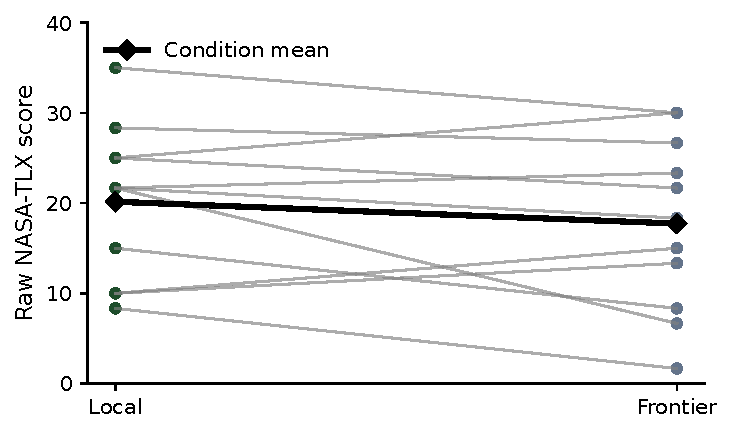
\includegraphics[width=0.65\linewidth]{figures/paired_workload.pdf}
    \caption{Within-participant Raw NASA-TLX scores under the 
    Local and Frontier conditions ($n=11$). Gray lines connect 
    individual participant scores, while the black line represents 
    the condition means. The vertical axis displays scores from 
    0 to 40 of the full 0--100 NASA-TLX scale.}
    \Description{Paired plot comparing individual participant
    workload scores under the Local and Frontier model-source
    conditions. Mean workload is slightly higher under the
    Local condition.}
    \label{fig:paired_workload}
\end{figure}

\subsection{Exploratory and Sensitivity Analyses}
An exploratory analysis examined whether model-source labels influenced participants' tendency to classify programming solutions as correct, regardless of actual solution correctness. Participants classified 16 of 24 Local-labeled solutions (66.67\%) as correct, compared with nine of 24 Frontier-labeled solutions (37.50\%), representing an observed difference of 29.17 percentage points. Figure~\ref{fig:evaluation_correctness} illustrates the distinction between evaluation accuracy and perceived correctness under both conditions. The Bayesian hierarchical logistic regression produced a posterior median odds ratio of 3.78, with a 95\% credible interval of [0.98, 15.86] and a posterior probability of a positive effect of 97.30\%. Although this represented the strongest directional evidence among the analyzed outcomes, the credible interval included an odds ratio of 1, and the finding remained exploratory.

Sensitivity analyses examined the influence of pilot participant inclusion and prior specification. Excluding the pilot participant did not substantially change the direction or interpretation of the estimated effects. The subjective workload analysis was unaffected because the pilot participant was already excluded from the complete-pair analysis. Under more restrictive prior distributions, the posterior median odds ratios decreased from 2.54 to 1.91 for evaluation accuracy, from 1.92 to 1.55 for evaluation confidence, and from 3.78 to 2.05 for perceived correctness. The posterior median workload difference decreased from 2.39 to 2.32 points. Although the direction of the estimated effects remained consistent across prior specifications, their magnitudes were sensitive to the degree of regularization, particularly for perceived correctness. All 95\% credible intervals continued to include their respective null values.

\begin{figure}[htbp]
    \centering
    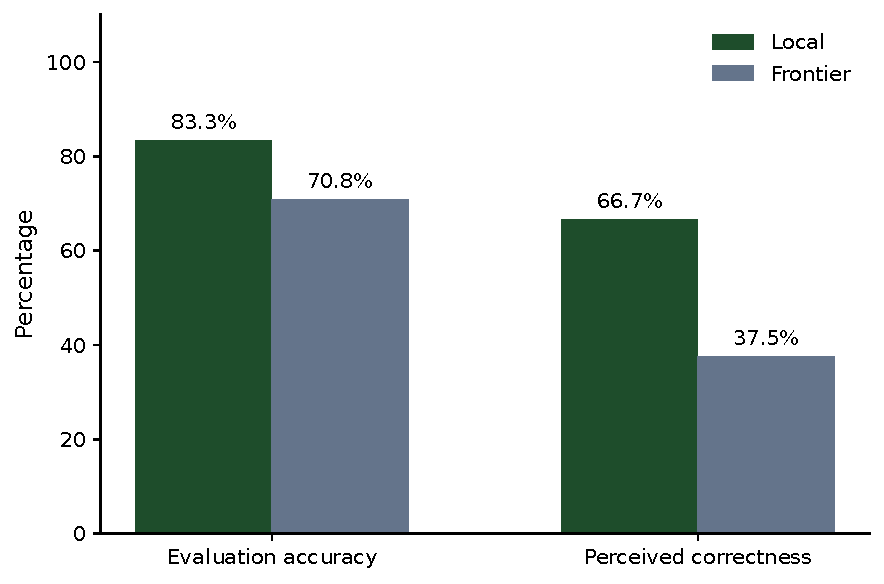
\includegraphics[width=0.75\linewidth]{figures/evaluation_correctness.pdf}
    \caption{Observed evaluation accuracy and perceived
    correctness rates under the Local and Frontier conditions,
    with 24 programming evaluations per condition.}
    \Description{Grouped bar chart comparing evaluation accuracy
    and perceived correctness under both model-source conditions.
    Both measures were higher under the Local condition.}
    \label{fig:evaluation_correctness}
\end{figure}

\subsection{Summary of Results and Model Diagnostics}

Across all three primary dependent measures, posterior estimates indicated higher values under the Local condition. However, none of the 95\% credible intervals excluded their respective null values. The exploratory analysis of perceived correctness provided the strongest directional evidence, although its estimated effect was sensitive to prior specification. Table~\ref{tab:bayesian_results} summarizes the posterior estimates, and Figure~\ref{fig:bayesian_effects} illustrates the estimated regression effects and their associated uncertainty.

All 11 retained Bayesian model fits produced zero divergent transitions, with satisfactory $\hat{R}$ statistics and effective sample sizes. Visual inspection of the trace plots indicated consistent mixing across sampling chains. Posterior predictive checks showed that the observed outcome means fell within the central regions of their corresponding predictive distributions. These diagnostics supported the numerical reliability of the posterior estimates.

\begin{table}[htbp]
    \centering
    \caption{Bayesian posterior effect estimates comparing the
    Local condition with the Frontier condition.}
    \label{tab:bayesian_results}
    \begin{tabular}{lrrr}
        \toprule
        \textbf{Outcome} &
        \textbf{Median} &
        \textbf{95\% CrI} &
        \textbf{P(Positive)} \\
        \midrule
        Accuracy (OR) & 2.54 & [0.61, 11.37] & 90.16\% \\
        Confidence (OR) & 1.92 & [0.62, 6.10] & 87.26\% \\
        Workload (points) & 2.39 & [-2.09, 6.59] & 87.74\% \\
        Perceived correctness (OR)$^*$ & 3.78 & [0.98, 15.86] & 97.30\% \\
        \bottomrule
    \end{tabular}

    \smallskip
    \footnotesize
    OR = odds ratio; CrI = credible interval.
    $^*$Exploratory outcome.
\end{table}

\begin{figure}[htbp]
    \centering
    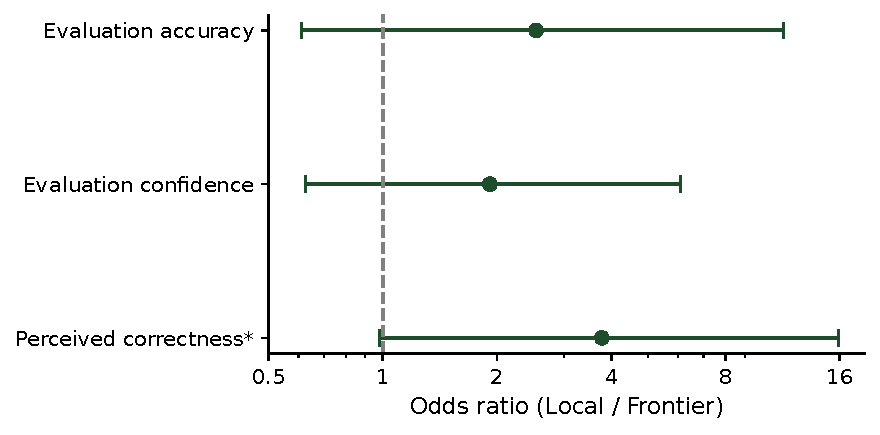
\includegraphics[width=0.75\linewidth]{figures/bayesian_effects.pdf}
    \caption{Posterior median odds ratios and 95\% credible
    intervals for the Local condition relative to the Frontier
    condition. The dashed vertical line represents an odds
    ratio of 1. The asterisk identifies the exploratory outcome.}
    \Description{Forest plot showing posterior median odds
    ratios and credible intervals for evaluation accuracy,
    evaluation confidence, and perceived correctness.
    All three credible intervals include an odds ratio of 1.}
    \label{fig:bayesian_effects}
\end{figure}

% --------------------------------------------------


% --------------------------------------------------
\section{Discussion}
% --------------------------------------------------


% --------------------------------------------------
\section{Conclusion}
% --------------------------------------------------

% --------------------------------------------------
\section{Use of AI}
Generative AI was used to assist with identifying relevant literature, organizing and revising the manuscript, and developing Python code for statistical analysis and visualization. All analyses were conducted locally by the author. The experimental design, data collection, methodological decisions, and final conclusions remained the responsibility of the author.


% --------------------------------------------------
% References
% --------------------------------------------------

\bibliographystyle{ACM-Reference-Format}
\bibliography{references}

\end{document}